% 
% simple.tex : part of the Mace toolkit for building distributed systems
% 
% Copyright (c) 2007, Charles Killian, Dejan Kostic, Ryan Braud, James W. Anderson, John Fisher-Ogden, Calvin Hubble, Duy Nguyen, Justin Burke, David Oppenheimer, Amin Vahdat, Adolfo Rodriguez, Sooraj Bhat
% All rights reserved.
% 
% Redistribution and use in source and binary forms, with or without
% modification, are permitted provided that the following conditions are met:
% 
%    * Redistributions of source code must retain the above copyright
%      notice, this list of conditions and the following disclaimer.
%    * Redistributions in binary form must reproduce the above copyright
%      notice, this list of conditions and the following disclaimer in
%      the documentation and/or other materials provided with the
%      distribution.
%    * Neither the names of Duke University nor The University of
%      California, San Diego, nor the names of the authors or contributors
%      may be used to endorse or promote products derived from
%      this software without specific prior written permission.
% 
% THIS SOFTWARE IS PROVIDED BY THE COPYRIGHT HOLDERS AND CONTRIBUTORS "AS IS"
% AND ANY EXPRESS OR IMPLIED WARRANTIES, INCLUDING, BUT NOT LIMITED TO, THE
% IMPLIED WARRANTIES OF MERCHANTABILITY AND FITNESS FOR A PARTICULAR PURPOSE ARE
% DISCLAIMED. IN NO EVENT SHALL THE COPYRIGHT OWNER OR CONTRIBUTORS BE LIABLE
% FOR ANY DIRECT, INDIRECT, INCIDENTAL, SPECIAL, EXEMPLARY, OR CONSEQUENTIAL
% DAMAGES (INCLUDING, BUT NOT LIMITED TO, PROCUREMENT OF SUBSTITUTE GOODS OR
% SERVICES; LOSS OF USE, DATA, OR PROFITS; OR BUSINESS INTERRUPTION) HOWEVER
% CAUSED AND ON ANY THEORY OF LIABILITY, WHETHER IN CONTRACT, STRICT LIABILITY,
% OR TORT (INCLUDING NEGLIGENCE OR OTHERWISE) ARISING IN ANY WAY OUT OF THE
% USE OF THIS SOFTWARE, EVEN IF ADVISED OF THE POSSIBILITY OF SUCH DAMAGE.
% 
% ----END-OF-LEGAL-STUFF----
\section{A Simple Example: Ping}
\label{sec:firstping}

As an introduction to Mace, we present a simple service that checks
the liveness of a peer by sending it ping messages.  A \emph{service}
is a piece of code with a well-defined interface that runs on one or
more distributed hosts and provides an implementation of the methods
(or services) specified by its interface.  For instance, a route
service provides methods and an implementation for routing messages to
a single host, and a multicast service provides methods and an
implementation for delivering a message to many hosts.  Services may
be used by other services as well as by applications.  This HOWTO will
show how to write a Ping service and a sample application using the
service.

Throughout the rest of this tutorial, all file paths are relative to
the \directory{mace} root directory.

\subsection{Ping Overview}
\label{sec:pingoverview}

\subsubsection{Usage Model}

Our ping application is designed to be run on two hosts.  One host is
the sender and the other is the responder.  The senders sends a
message to the responder, who then sends a response message back to
the sender.  The sender will print that it received a response, or
will report an error if it times out.

In \S~\ref{sec:ping}, we show how to extend our usage model to support
multiple hosts, continuous queries, and more detailed latency reports.

\subsubsection{Application and Service Components}

%% Our ping application will involve writing the following components, 
%% illustrated in Figure \ref{fig:ping_structure}:

%% %XXX: Figures and docbook?
%% \begin{figure}[t]
%% \begin{center}
%% 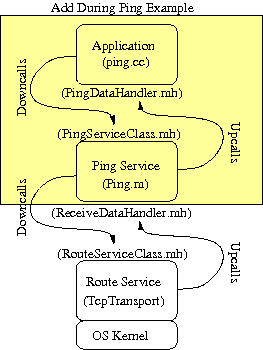
\includegraphics{ping_structure}
%% \caption{\small{Structure of the Ping example.  The parts which are 
%%   written during the example are in the shaded box.}}
%% \label{fig:ping_structure}
%% \end{center}
%% \end{figure}

\begin{description}

\item[Service Class Definition: \filename{PingServiceClass.mh}]
  \S~\ref{sec:serviceclass-def}-\S~\ref{sec:serviceclassnotes}.
  The interface for our service, defined in a Mace service class
  header file.

\item[Handler Definition: \filename{PingDataHandler.mh}]
  \S~\ref{sec:handler-def}-\S~\ref{sec:datahandlernotes}.  The interface for
  receiving upcalls\footnote{upcalls are the Mace lingo for callbacks.  They
  are called upcalls because they are calls from lower levels of services to
  upper layers} from our service, defined in a Mace handler class header file.

\item[Service Implementation: \filename{(First)Ping.mac}]
  \S~\ref{sec:service-implementations}-\S~\ref{sec:first-ping-implementation}.
  The actual implementation of our Ping service, written using the
  Mace language in a Mace service file.

\item[Application: \filename{(first)ping.cc}]
  \S~\ref{sec:first-ping-application}.  The implementation of the ping
  application.  The application 1) instantiates a service instance and
  a handler instance, 2) registers the handler with the service, and
  3) runs the service.  This is a standard C++ file/application.

\end{description}


\subsection{ServiceClass Definitions}
\label{sec:serviceclass-def}

Before implementing the application, we will first design the interface the
application will use so that the application and the service may be written
independently.  The way to do this in Mace is by writing a service class and
optionally one or more handlers, which are classes that receive upcalls
(\emph{i.e.} callbacks) for event notifications.

All Mace services implement one or more \emph{service classes}, which
are specifications of the API provided by the service.  Service
classes are analogous to \emph{interfaces} in Java.  Service classes
are defined in Mace header files, with names of the form
\replaceable{ServiceName}\filename{ServiceClass.mh}.  Service class
header files should be placed in \directory{services/interfaces}.  (Mace
includes a variety of service classes, which are listed in
\S~\ref{sec:service-classes}.)  We first present our example service
class and then describe some of the details
(\S~\ref{sec:serviceclassnotes}):

\subsection{PingServiceClass}
\label{sec:pingserviceclass}

The service class definition \filename{services/interfaces/PingServiceClass.mh}
follows:

\lgrindfile{PingServiceClass.mh}

The Ping service provides two methods:

\begin{description}

\item[\function{monitor}] Request that the service monitor a new host.

\item[\function{getLastResponseTime}] Query the service for the last time, in
  epoch microseconds, that a response was received from the given
  host.

\end{description}

The Ping service also has one upcall handler, of type
\classname{PingDataHandler}.  Handlers will be described in more
detail later.

The type \typename{MaceKey} is a class used to represent the address
of a host.  For our simple application, these simply represent IPv4
addresses.  However, \typename{MaceKey}s can also represent other
classes of addresses, such as SHA1 160~bit hashes, which are used by
overlay routing protocols such as Chord and Pastry (which is why they
are named \emph{keys}).


\subsection{ServiceClass Notes}
\label{sec:serviceclassnotes}

The Mace service header files are very similar to C++ header files.
They are, in fact, automatically translated into C++ header files by
the build process.  Here are some notes to keep in mind when writing
service class header files.

\begin{description}

\item[\symbolkw{\#ifndef ... \#define ... \#endif}] These necessary
  preprocessor directives to prevent a file from being included twice
  are automatically generated for the C++ header file.  Do not include
  them in your \filename{.mh} Mace service header file.

\item[\symbolkw{\#include}, declarations, typedefs, etc] All code
  between the start of the \filename{.mh} file and the class
  declaration is copied verbatim into the generated C++ header file.
  Put appropriate \symbolkw{\#include} directives here.

\item[Class declaration and inheritance] All service classes inherit
  from the base class \classname{ServiceClass}.  A ServiceClass may
  extend other ServiceClasses, but all ServiceClasses have
  \classname{ServiceClass} as a common ancestor.  If no service
  classes are listed as super classes, then the generated C++ header
  file will have \classname{ServiceClass} listed as the sole super
  class.  Derived service classes inherit from other service classes
  using the normal C++ syntax.  However, all super service classes
  must be specified with no modifies (\symbolkw{public},
  \symbolkw{virtual}, etc).  For instance, the service class declaration for
  \classname{OverlayRouterServiceClass} is:

\begin{programlisting}
serviceclass OverlayRouterServiceClass : OverlayServiceClass { ... 
\end{programlisting}

  To define a handler instead of a service class, use the keyword
  \symbolkw{handler} instead.

\item[Method implementations] All service class methods must have an
  implementation.  If desired, a default implementation may be
  provided in the service header file (as done for
  \function{getLastResponseTime}), which will be copied verbatim into
  the generated C++ header file.  If no method implementation is
  provided, then a default implementation will be generated that
  will \function{assert} failure.

\item[\symbolkw{handlers}] Mace service header files introduce a new
  keyword, \symbolkw{handlers}, that declares the handlers used by the
  service.  Recall that handlers are classes (also defined in
  \filename{.mh} files, described in detail in the next section) that
  receive upcalls for event notifications.  \symbolkw{handlers}
  should be followed by a comma separated list of one or more handler
  names, followed by a semicolon.  Thus, we are declaring that
  \classname{PingServiceClass} has one handler, of type
  \classname{PingDataHandler}.

  The \symbolkw{handlers} declaration will cause four methods,
  \function{registerHandler}, \function{registerUniqueHandler},
  \function{unregisterHandler}, and \function{unregisterUniqueHandler} to be
  generated for each handler listed.  These methods are the means by which
  actual handler objects are registered and unregistered with the service to
  receive upcalls when the service has an event to report.  For example, the
  Ping service will report when it receives a response from a monitored host or
  when it times out waiting for an expected response.

  Calling \function{registerHandler} allows you to register multiple upcall
  handlers for a single service instance.  This is illustrated later in
  \S~\ref{sec:ping-application}.  The \function{registerUniqueHandler} method
  tells the service that you are registering exactly one upcall
  handler\footnote{In truth, it simply registers your handler with a
  pre-defined and well-known id which only one handler may be associated
  with.}.  We use this in our first Ping application in
  \S~\ref{sec:first-ping-application}.

\item[Registration IDs] In the generated header file, all method
  signatures will be modified so that they take an additional parameter of type
  \typename{registration\_uid\_t} as the last argument that is assigned a
  default value of \literal{-1}.  Registration IDs are not needed by
  application writers when you register unique handlers.  You do not need to
  worry about registration IDs right now; we mention this for the sake of
  completeness.

\end{description}


\subsection{Handler Definitions}
\label{sec:handler-def}

Many Mace services provide the option to register objects to receive
upcalls for event notifications (declared by using the
\symbolkw{handlers} keyword).  To make a method upcall, a service
needs an object, with a well-defined interface, on which to make the
method call: this object is the \emph{handler}.  Handler objects
implement a single \emph{handler class} interface.  Handler classes
are analogous to service classes: they provide API specifications.
The APIs for the upcall methods are defined in Mace header files
with names of the form \replaceable{HandlerType}\filename{Handler.mh}.
Handler class definition header files should also be placed in
\directory{services/interfaces}.

\subsection{PingDataHandler}
\label{sec:pingdatahandler}

The handler class definition for
\filename{services/interfaces/PingDataHandler.mh} follows:

\lgrindfile{PingDataHandler.mh}

The Ping data handler provides two methods:

\begin{description}

\item[hostResponseReceived] Upcall indicating that the given host
  responded to a ping message.  The four parameters are: 1) the host
  that responded, 2) the time we sent the ping message, 3) the time we
  received the ping reply, and 4) the time the remote host sent the
  ping reply.

\item[hostResponseMissed] Upcall indicating that the given host
  failed to respond to a ping message within the timeout period.

\end{description}

\subsection{Handler Notes}
\label{sec:datahandlernotes}

All the notes for ServiceClass definitions, described in
\S~\ref{sec:serviceclassnotes}, apply for handlers, except for 1) the
requirement to extend from a base service class: handlers need not and
should not inherit from any super class, and 2) the \symbolkw{handlers}
declaration may not be used in handler classes, only service classes.

\subsection{Service Implementations}
\label{sec:service-implementations}

Services are implemented in subdirectories of \directory{services}.
Typically, services are implemented in files with names of the form
\classname{ServiceName}\filename{.mac}, under the subdirectory
\directory{services/}\classname{ServiceName}.

%%%%%%%%%%%%%%%%%%%%%%%%%%%%%%%%%%%%%%%%%%%%%%%%%%%%%%%%%%%%%%%%%%%%%%%%
% First Ping
%%%%%%%%%%%%%%%%%%%%%%%%%%%%%%%%%%%%%%%%%%%%%%%%%%%%%%%%%%%%%%%%%%%%%%%%

\subsection{Ping Implementation}
\label{sec:first-ping-implementation}

We are now ready to implement our Ping service.  First, create the new
directory \directory{services/Ping}.

The implementation of \filename{services/Ping/FirstPing.mac} follows:

\lgrindfile{FirstPing.mac}


For a detailed discussion of the Mace language, see
\S~\ref{sec:firstping-detail}.  We will now describe how to
compile the service and write a simple application that uses the
service.

\subsubsection{Compiling the Ping Service}
\label{sec:compiling-ping-m}

Edit \filename{services/CMakeLists.txt}, and add \literal{Ping} to the
list of services specified in the \variablename{SERVICE\_DIRS}
variable\footnote{Note that this is the name of the directory, not the
name of the service, so if you used a name other than `Ping' for the
directory, you should use that here}.  Then you can go to the configured
builds directory, and run \command{make Ping}, which will re-run CMake,
and build the Ping service directory library.


\subsection{Ping Application}
\label{sec:first-ping-application}

We will now write a simple application that uses the Ping service.
Our application will report the round-trip response time latency for
live hosts, or will report that the given host is not responding.

Create the new directory \directory{applications/ping} for our program.

We implement our program in \filename{applications/ping/firstping.cc} as
follows:

\lgrindfile{firstping.cc}

A brief overview of this file:

\begin{enumerate}

\item We define \classname{PingResponseHandler}, which inherits from
  \classname{PingDataHandler}, and overrides both methods.

\item In \function{main()}, we instantiate a
  \classname{PingResponseHandler} and a \classname{PingServiceClass}.

\item We call \function{maceInit()} on our Ping service object, which
  initializes the service state, and also executes the
  \function{downcall~maceInit} transition, if defined (we did not define one).

\item We register our \classname{PingResponseHandler} with our service
  instance as a unique handler.  The \function{registerUniqueHandler}
  method indicates that there will be only one handler of that type
  registered with the service.  The implication of this is that
  registration IDs will not be needed to differentiate handlers.

\item When run with no arguments, the program will simply respond to
  other ping requests with ping replies.  As a responder, the program
  will loop forever in the \function{select}.

\item When run with a single argument, \command{ping} will send a
  single ping message to the given host, and either print the
  round-trip latency or report that it did not receive a response.
  The handler callback methods call \function{exit()}, so the program
  will then terminate.

\end{enumerate}

Because the Mace runtime libraries use threads, it is important that
\function{main()} does not exit until the services complete their
tasks.  Thus, we recommend calling \function{SysUtil::sleep()} with
no arguments, which is an efficient way to ensure that the main thread
does not cause the process to exit.

\subsubsection{Compiling firstping.cc}
\label{sec:compiling-ping-cc}

We need to write a very simple CMakeLists.txt to tell CMake how to build
our program.  The CMakeLists.txt
\filename{applications/ping/CMakeLists.txt} follows:

\verbatiminput{CMakeLists.txt.firstping}

Also, we need to tell CMake to include the ping application directory.
To do so, edit \filename{applications/CMakeLists.txt}, and add the line
\literal{ADD\_SUBDIRECTORY(ping)}.  Then, go to the \directory{builds}
directory, and run \command{make firstping}, which will build the
firstping application at \filename{builds/application/ping/firstping}.

\subsection{Running Ping}
\label{sec:running-ping}

Copy the \filename{firstping} executable to another machine.  Assuming your
two machines are named \replaceable{alexander} and \replaceable{philip}, run the
following commands.

\noindent
On \replaceable{philip}:

\begin{screen}
\command{philip$ ./firstping}
\end{screen}
%$

\noindent
On \replaceable{alexander}:

\begin{screen}
\command{alexander$ ./firstping philip}
IPV4/philip(192.168.0.2) responded in 503404 usec
\end{screen}
%$

\noindent
Now kill the \command{firstping} process on \replaceable{philip}.  Re-run
the command on \replaceable{alexander}:

\small
\begin{screen}
\command{alexander$ ./firstping philip}
did not receive response from IPV4/philip(192.168.0.2) pinged at Mon May  9 22:01:14 2005
\end{screen}
%$
\normalsize

\noindent
Congratulations!  You have written your first Mace service and
application.

